\usetikzlibrary{matrix,backgrounds,positioning,calc,fit}
\definecolor{SceneColor}{RGB}{200,200,200}
\definecolor{GroupColor}{RGB}{90,200,102}
\definecolor{SubGroupColor}{RGB}{114,247,247}

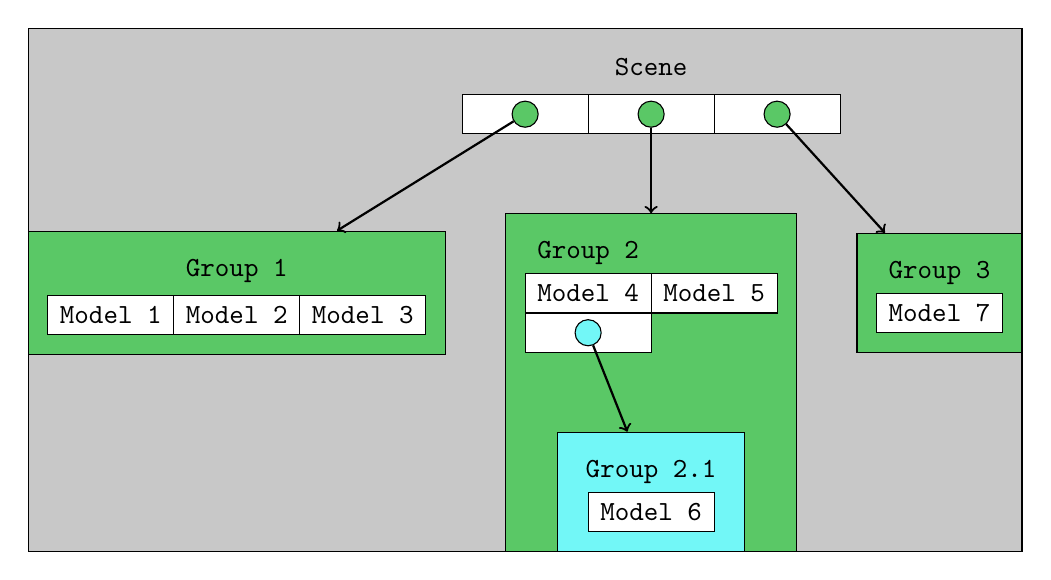
\begin{tikzpicture}[font=\ttfamily,
    array/.style={matrix of nodes,
    nodes={draw, minimum width=16mm, minimum height=5mm, fill=white},
    column sep=-\pgflinewidth,
    row sep=-\pgflinewidth,
    nodes in empty cells,
    row 1/.style={nodes={draw=none, fill=none, minimum size=5mm}}}]

    \matrix[array] (Scene) {
        & Scene & \\
        &  &    \\
    };

    \matrix[array, below = of Scene] (Group2) {
        Group 2 \\
        Model 4 & Model 5 \\
        \\
    };

    \matrix[array, left = of Group2] (Group1) {
        &  Group 1 & \\
        Model 1 & Model 2 & Model 3 \\
    };

    \matrix[array, right = of Group2] (Group3) {
        Group 3 \\
        Model 7 \\
    };

    \matrix[array, below = of Group2] (Group21) {
        Group 2.1 \\
        Model 6 \\
    };

    \node[draw, fill=GroupColor, minimum size=2mm, circle] at (Scene-2-1) (Group1Ball) {};
    \node[draw, fill=GroupColor, minimum size=2mm, circle] at (Scene-2-2) (Group2Ball) {};
    \node[draw, fill=GroupColor, minimum size=2mm, circle] at (Scene-2-3) (Group3Ball) {};
    \node[draw, fill=SubGroupColor, minimum size=2mm, circle] at (Group2-3-1) (Group21Ball) {};

    \begin{scope}[on background layer]
        \node[draw, fill=SceneColor, fit = (Scene) (Group1) (Group2) (Group3) (Group21)]
        (SceneBox) {};
        \node[draw, fill=GroupColor, fit = (Group1)] (Group1Box) {};
        \node[draw, fill=GroupColor, fit = (Group2) (Group21)] (Group2Box) {};
        \node[draw, fill=GroupColor, fit = (Group3)] (Group3Box) {};
        \node[draw, fill=SubGroupColor, fit = (Group21)] (Group21Box) {};
    \end{scope}

    \foreach \from/\to in {
        Group1Ball/Group1Box, Group2Ball/Group2Box,
        Group3Ball/Group3Box, Group21Ball/Group21Box}
    \draw [->, thick] (\from)--(\to);

\end{tikzpicture}
